\documentclass[11pt]{article}

\usepackage{geometry}
\geometry{letterpaper}
\usepackage{amsmath}
\usepackage{graphicx} % more modern
\usepackage{subfig}


\def\E{{\rm E}}
\def\Var{{\rm Var}}
\def\I{{\bf I}}
\def\w{{\bf w}}
\def\B{{\bf B}}
\def\b{{\bf b}}
\def\a{\alpha}
\def\tI{\tilde{\bf I}}
\def\tM{\tilde{M}}

\def\bF{{\bar{F}}}
\def\F{{\bf F}}

\def\D{{\cal D}}
\def\C{{\cal C}}
\def\S{{\cal S}}
\def\L{{\cal L}}

\def\obs{{\rm obs}}
\def\syn{{\rm syn}}

\begin{document}

\title{Deep FRAME model experiment}
	
\section{Deep FRAME Model}
To fix notation, let $\I(x)$ be an image defined on the square (or rectangular) image domain $\D$, where $x = (x_1, x_2)$ indexes the coordinates of pixels. We can treat $\I(x)$ as a two-dimensional function defined on $\D$. We can also treat $\I$ as a vector if we fix an ordering for the pixels. 

For a filter $F$, let $F*\I$ denote the filtered image or feature map, and let $[F*\I](x)$ denote the filter response or feature at position $x$. 

A deep FRAME model is a composition of multiple layers of linear filtering and element-wise non-linear transformation as expressed by the following recursive formula: 
\begin{equation}
	%\begin{aligned}
	[F^{(l)}_{k}  *\I](x)  =   h\left(\sum_{i=1}^{N_{l-1}}  \sum_{y \in \S_{l}} w^{(l, k)}_{i, y}   [F^{(l-1)}_{i}*\I](x+y) + b_{l, k}\right) \\
	%\end{aligned}
	\label{eq:ConvNet}
\end{equation}
where $l \in \{1, 2, ..., {\cal L}\}$ indexes the layer.  $\{F^{(l)}_k, k = 1, ..., N_l\}$ are the filters at layer $l$, and $\{F^{(l-1)}_i, i = 1, ..., N_{l-1}\}$ are the filters at layer $l-1$.  $k$ and $i$ are used to index filters at layers $l$ and $l-1$ respectively, and $N_l$ and $N_{l-1}$ are the numbers of filters at layers $l$ and $l-1$ respectively. The filters are locally supported, so the range of $y$  is within a local support $\S_{l}$  (such as a $7 \times 7$ image patch). At the bottom layer, $[F^{(0)}_k*\I](x) = \I_k(x)$, where $k \in \{R, G, B\}$ indexes the three color channels. Sub-sampling may be implemented so that in  $[F^{(l)}_{k}  *\I](x)$, $x \in \D_l \subset \D$. 

We take $h(r) = \max(r, 0)$, the rectified linear unit (re-lu), that is commonly adopted in modern ConvNet. We define the following random field model as the deep FRAME model:
\begin{equation}
p(\I; w) = \frac{1}{Z(w)} \exp \left[\sum_{k=1}^{K} \sum_{x \in {\cal D}_L} [F_k^{(L)}*\I](x)\right] q(\I), 
\label{eq:ConvNet-FRAME}
\end{equation}
where $b_k$ is the bias term, $w = (w_k, b_k, k = 1, ..., K)$, and $h(r) = \max(r, 0)$. $q(\I)$ is the Gaussian white noise model.

Model (\ref{eq:ConvNet-FRAME})  corresponds to the exponential tilting model with scoring function
\begin{equation}
f(\I; w) = \sum_{k=1}^{K} \sum_{x \in {\cal D}_L} [F_k^{(L)}*\I](x). \label{eq:a}
\end{equation}

The learning of $w$ from training images $\{\I_m, m = 1, ..., M\}$ can be accomplished by maximum likelihood. Let $L(w) = \sum_{m=1}^{M} \log p(\I; w)/M$, 
\begin{equation}
	%\begin{aligned}
	\frac{\partial L(w)}{\partial w} = \frac{1}{M} \sum_{m=1}^{M} \frac{\partial}{\partial w} f(\I_m; w) 
	-  \E_{w} \left[ \frac{\partial}{\partial w} f(\I; w) \right].
	%\end{aligned}
\end{equation}


The expectation can be approximated by Monte Carlo samples. One can sample from $p(\I; w)$ in (\ref{eq:ConvNet-FRAME}) by the Langevin dynamics: 
\begin{equation}
\I_{\tau+1} = \I_{\tau} - \frac{\epsilon^2}{2} \left[\I_\tau - \frac{\partial}{\partial \I}f(\I; w) \right] + \epsilon Z_\tau,
\end{equation}
where $\tau$ denotes the time step, $\epsilon$ denotes the step size, assumed to be sufficiently small, $Z_\tau \sim {\rm N}(0, {\bf 1})$.

We can build up the model layer by layer. 
Given the filters at layers below, the top layer weight and bias parameters can be learned according to 
\begin{equation}
\begin{aligned}
\frac{\partial L(w)}{\partial w_{i, y}^{(L, k)}} =& \frac{1}{M} \sum_{m=1}^{M}\sum_{x \in {\cal D}_L} \delta^{(L)}_{k, x}(\I_m; w)  [F^{(L-1)}_{i} * \I_m](x+y) \\
&   -  \frac{1}{\tilde{M}} \sum_{m=1}^{\tilde{M}} \sum_{x \in {\cal D}_L} \delta^{(L)}_{k, x}(\tilde{\I}_m; w)  [F^{(L-1)}_{i} * \tilde{\I}_m](x+y), \\
\end{aligned}
\label{eq:generativeGradient}
\end{equation}
and
\begin{equation}
\begin{aligned}
\frac{\partial L(w)}{\partial b_{L, k}} = \frac{1}{M} \sum_{m=1}^{M}\sum_{x \in {\cal D}_L} \delta^{(L)}_{k, x}(\I_m; w) - \frac{1}{\tilde{M}} \sum_{m=1}^{\tilde{M}} \sum_{x  \in {\cal D}_L} \delta^{(L)}_{k, x}(\tilde{\I}_m; w).
\end{aligned}
\label{eq:generativeGradient0}
\end{equation}
where $\I_m$ are $M$ observed images, and $\tilde{\I}_m$ are $\tilde{M}$ synthesized images sampled from the model.

\section{Experiment}
For each input image, design a set of filters, and learn a Deep FRAME model. We define the Julesz ensemble as the set of images that reproduce the observed sufficient statistics over those designed filters. You use Langevin dynamics to draw samples from the model. Figure~\ref{fig:syn} shows an example of synthesis. The synthesis starts from a zero image and the sampling stops when it matches all the sufficient statistics. To reduce the computational complexity, all images are resized into the size of $224\times224$ pixels.

\begin{figure}[h]
	\centering
	\setlength{\fboxrule}{1pt}
	\setlength{\fboxsep}{0cm}	
	\subfloat{
		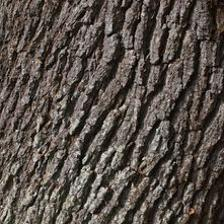
\includegraphics[width=.16\linewidth]{./image/bark.jpg}
		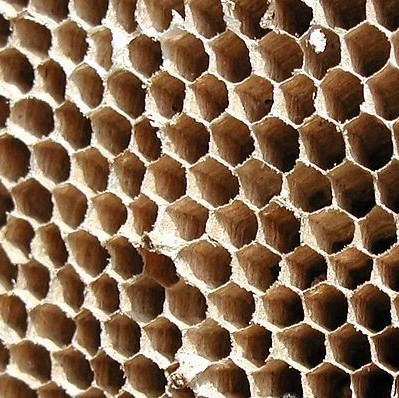
\includegraphics[width=.16\linewidth]{./image/beehive.jpg}
		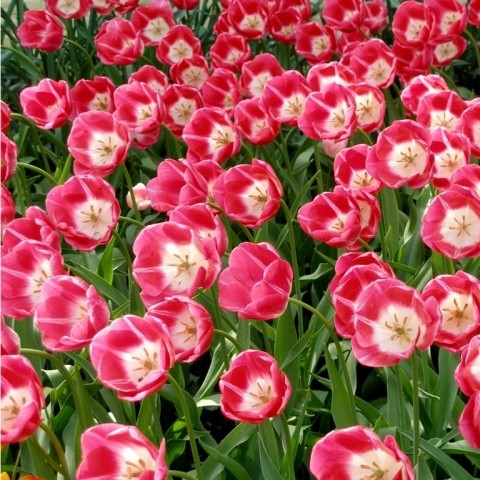
\includegraphics[width=.16\linewidth]{./image/rose.jpg}
		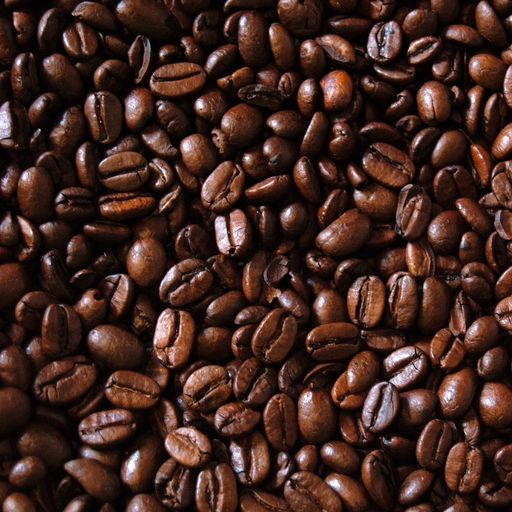
\includegraphics[width=.16\linewidth]{./image/coffee.jpg}
		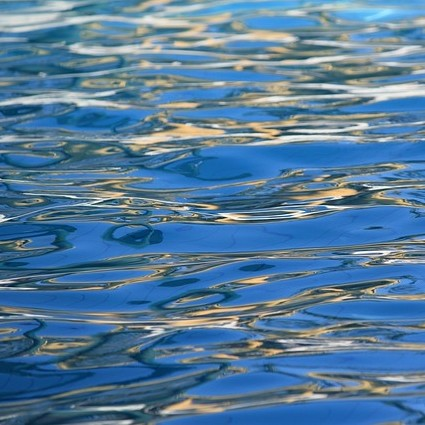
\includegraphics[width=.16\linewidth]{./image/water.jpg}
		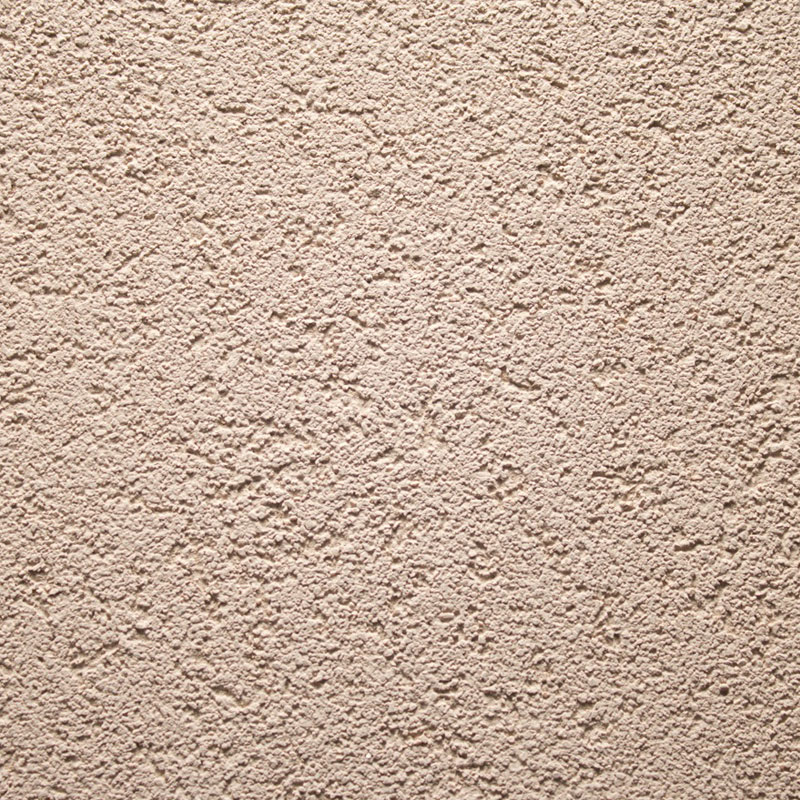
\includegraphics[width=.16\linewidth]{./image/stucco.jpg}
	}\\[3px]
	\caption{Six training images.}
\end{figure}

\begin{figure}[h]
	\centering
	\setlength{\fboxrule}{1pt}
	\setlength{\fboxsep}{0cm}	
	\subfloat{
		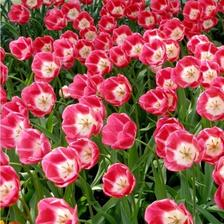
\includegraphics[width=.22\linewidth]{./image/rose_small.jpg}
		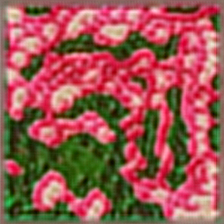
\includegraphics[width=.22\linewidth]{./image/layer_1.png}
		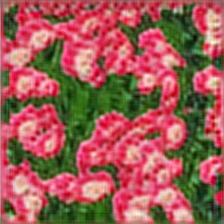
\includegraphics[width=.22\linewidth]{./image/layer_2.png}
		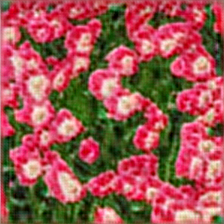
\includegraphics[width=.22\linewidth]{./image/layer_3.png}
	}\\[3px]
	\caption{Synthesis example. The first image is the training image, and from left to right, the rest images are synthesized images using one layer to three layers respectively.}
	\label{fig:syn}
\end{figure}

\section{Code}
The code locates at  \verb|.\release\|, and training images locates at \verb|.\Image\|. The synthesized results will be saved at \verb|.\release\synthesiedImage\|, and the model will be saved at \verb|.\release\working\|.

1. \verb|experiment_learn_frame.m| is the main entry function, which gives an example of learning and synthesizing images from the model. \textbf{Modification:} You need to write your own main function to do experiment on all six images.

2. \verb|add_bottom_filters.m| is the function to design the structure of Deep FRAME model. \textbf{Modification:} You design your own structure of the model. The example setting may not generate vivid results. You can use more filters and larger sub-sampling size for each filter. You can also try a model with more layers to generate more realistic images. Specifically, you can modify the following parameters:

a) \verb|num_in|: Number of filters in the previous layer.

b) \verb|num_out|: Number of filters in the current layer.

c) \verb|stride|: Sub-sampling size for each filter. For instance, when stride = 2, the convolution for each filter is computed every two pixels. 

d) \verb|filter_sz|: Filter size in pixel, and we use square filters. Note that the filter size is the size defined on feature map $F*\I$. Here is one example to compute the filter size in the second layer. Suppose in the first layer, \verb|filter_sz = 5, stride = 2|, and in the second layer \verb|filter_sz = 3|, then the filter size in the second layer can be computed by $(3-1)\times 2 + 5 = 9$

3. \verb|train_model_generative.m| is the function to learn model and synthesize images.

4. \verb|visualize_filters.m| is the function to visualize filters in the first layer. \textbf{Modification:} Write you own function to visualize filters in the first layer. The learned filters in the first layer is saved in \verb|net.layers{1}.weights{1}|.

To run the code, you need firstly to run \verb|Setup.m| to configure and compile the code. You can either use CPU or GPU version. To use GPU, set \verb|config.gpus = [1]| in \verb|frame_config.m|, otherwise, set \verb|config.gpus = []|.

\section{Submission}
There are two tasks, 

1. Show the synthesized images from each layer.

2. Display the filters in the first layer using your \verb|visualize_filters.m|.


	
\end{document}